\documentclass[11pt]{article}
\usepackage[margin=1in]{geometry}
\usepackage{amsmath}
\usepackage{amssymb}
\usepackage[utf8]{inputenc} 
\usepackage{graphicx} 
\usepackage{parskip} 
\usepackage{multirow} 
\usepackage{mathtools}

\DeclarePairedDelimiter\abs{\lvert}{\rvert}%
\DeclarePairedDelimiter\norm{\lVert}{\rVert}%

\makeatletter
\let\oldabs\abs
\def\abs{\@ifstar{\oldabs}{\oldabs*}}

\let\oldnorm\norm
\def\norm{\@ifstar{\oldnorm}{\oldnorm*}}
\makeatother
\usepackage{multicol} 
\usepackage[spanish,es-nodecimaldot]{babel} 
\usepackage{mathtools}
\usepackage{amsfonts}
\usepackage{float}
\usepackage{textcomp}
\usepackage{caption}
\usepackage{subfig}
\usepackage[spanish]{babel}
\usepackage{gensymb}
\def\sen{\mathop{\mbox{\normalfont sen}}\nolimits}

\usepackage{fancyhdr}
\fancyhf{}
\rfoot{\thepage}
\pagestyle{fancy}
\lhead{Nieto Castellanos Fabián}
\chead{}
\rhead{Tarea 10. Histogramas}
\begin{document}

\textbf{1)}
\begin{figure}[H]
\centering
\subfloat[]{
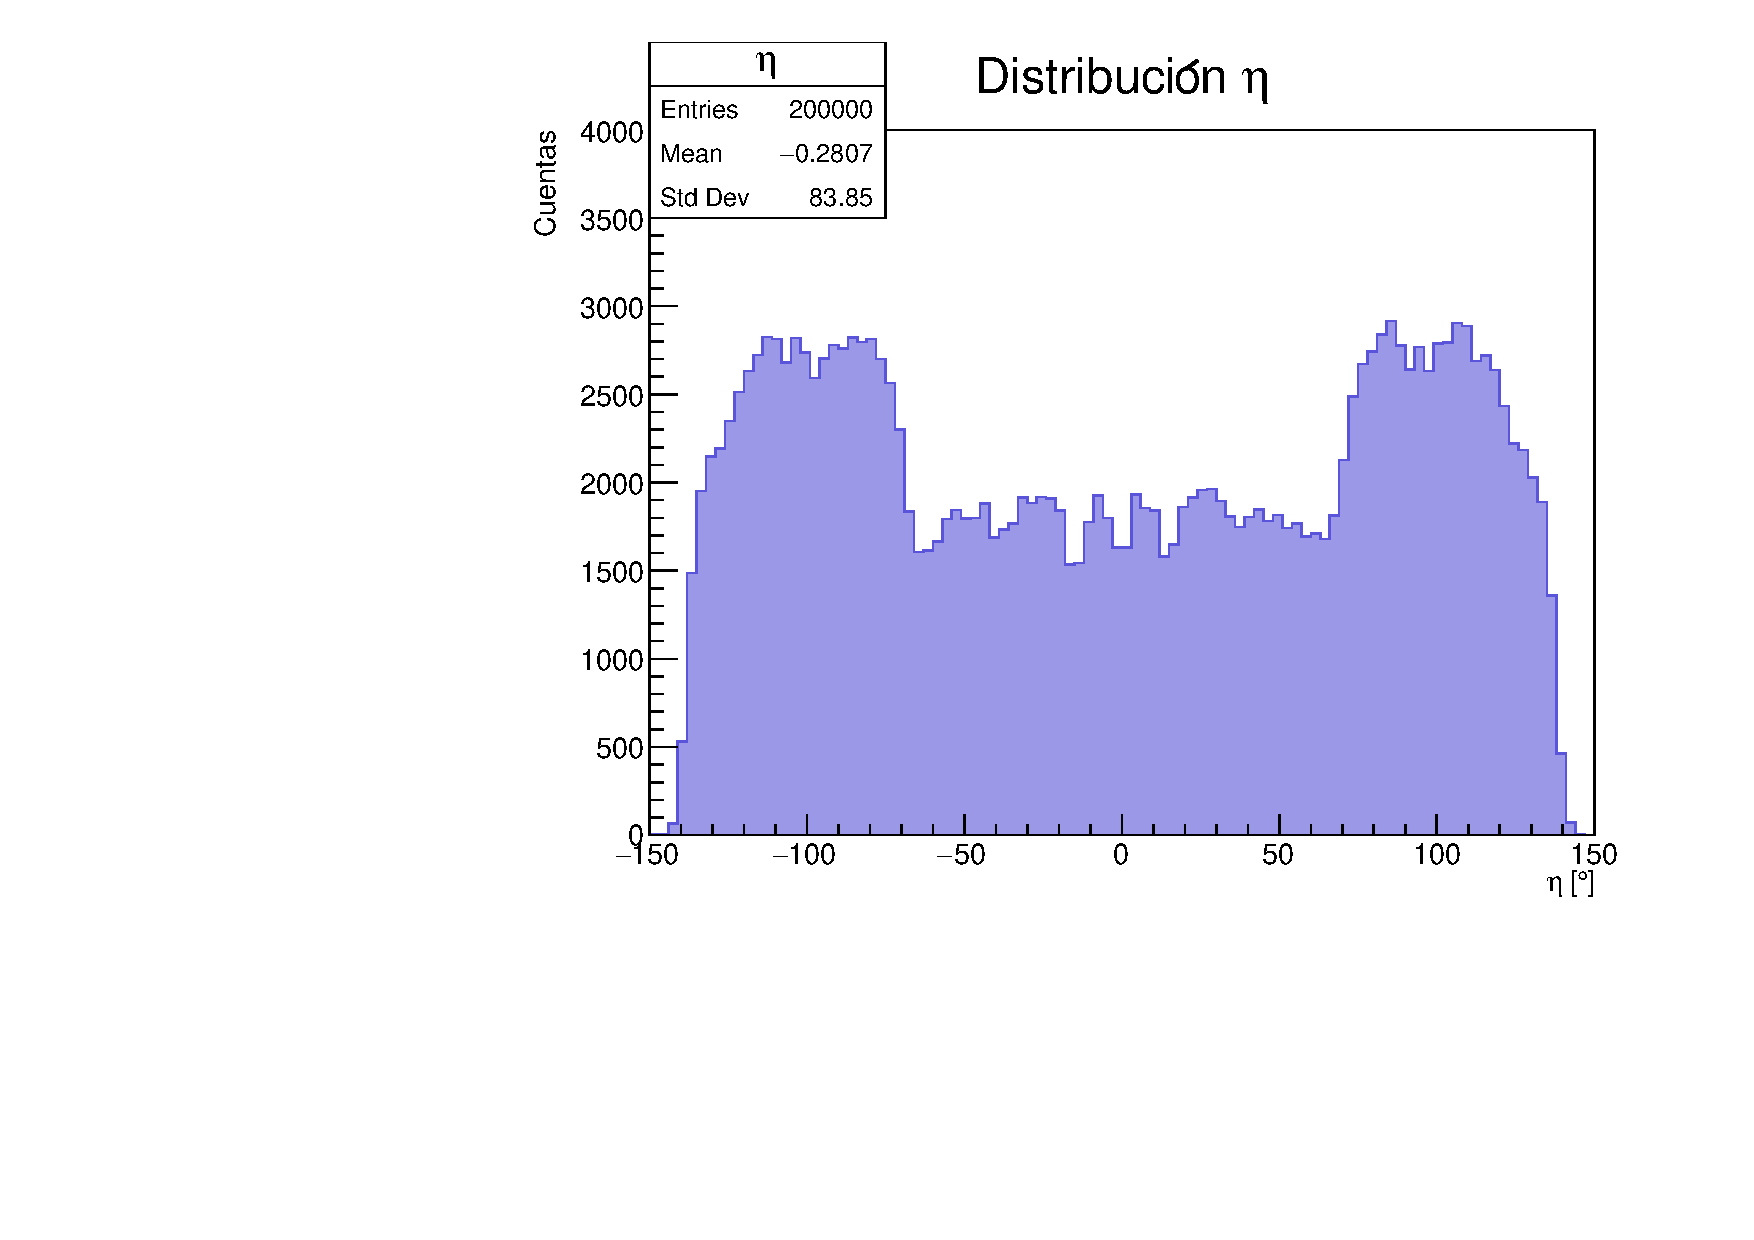
\includegraphics[width=0.8\textwidth]{../Figuras/Prob1A.pdf}}

\subfloat[]{
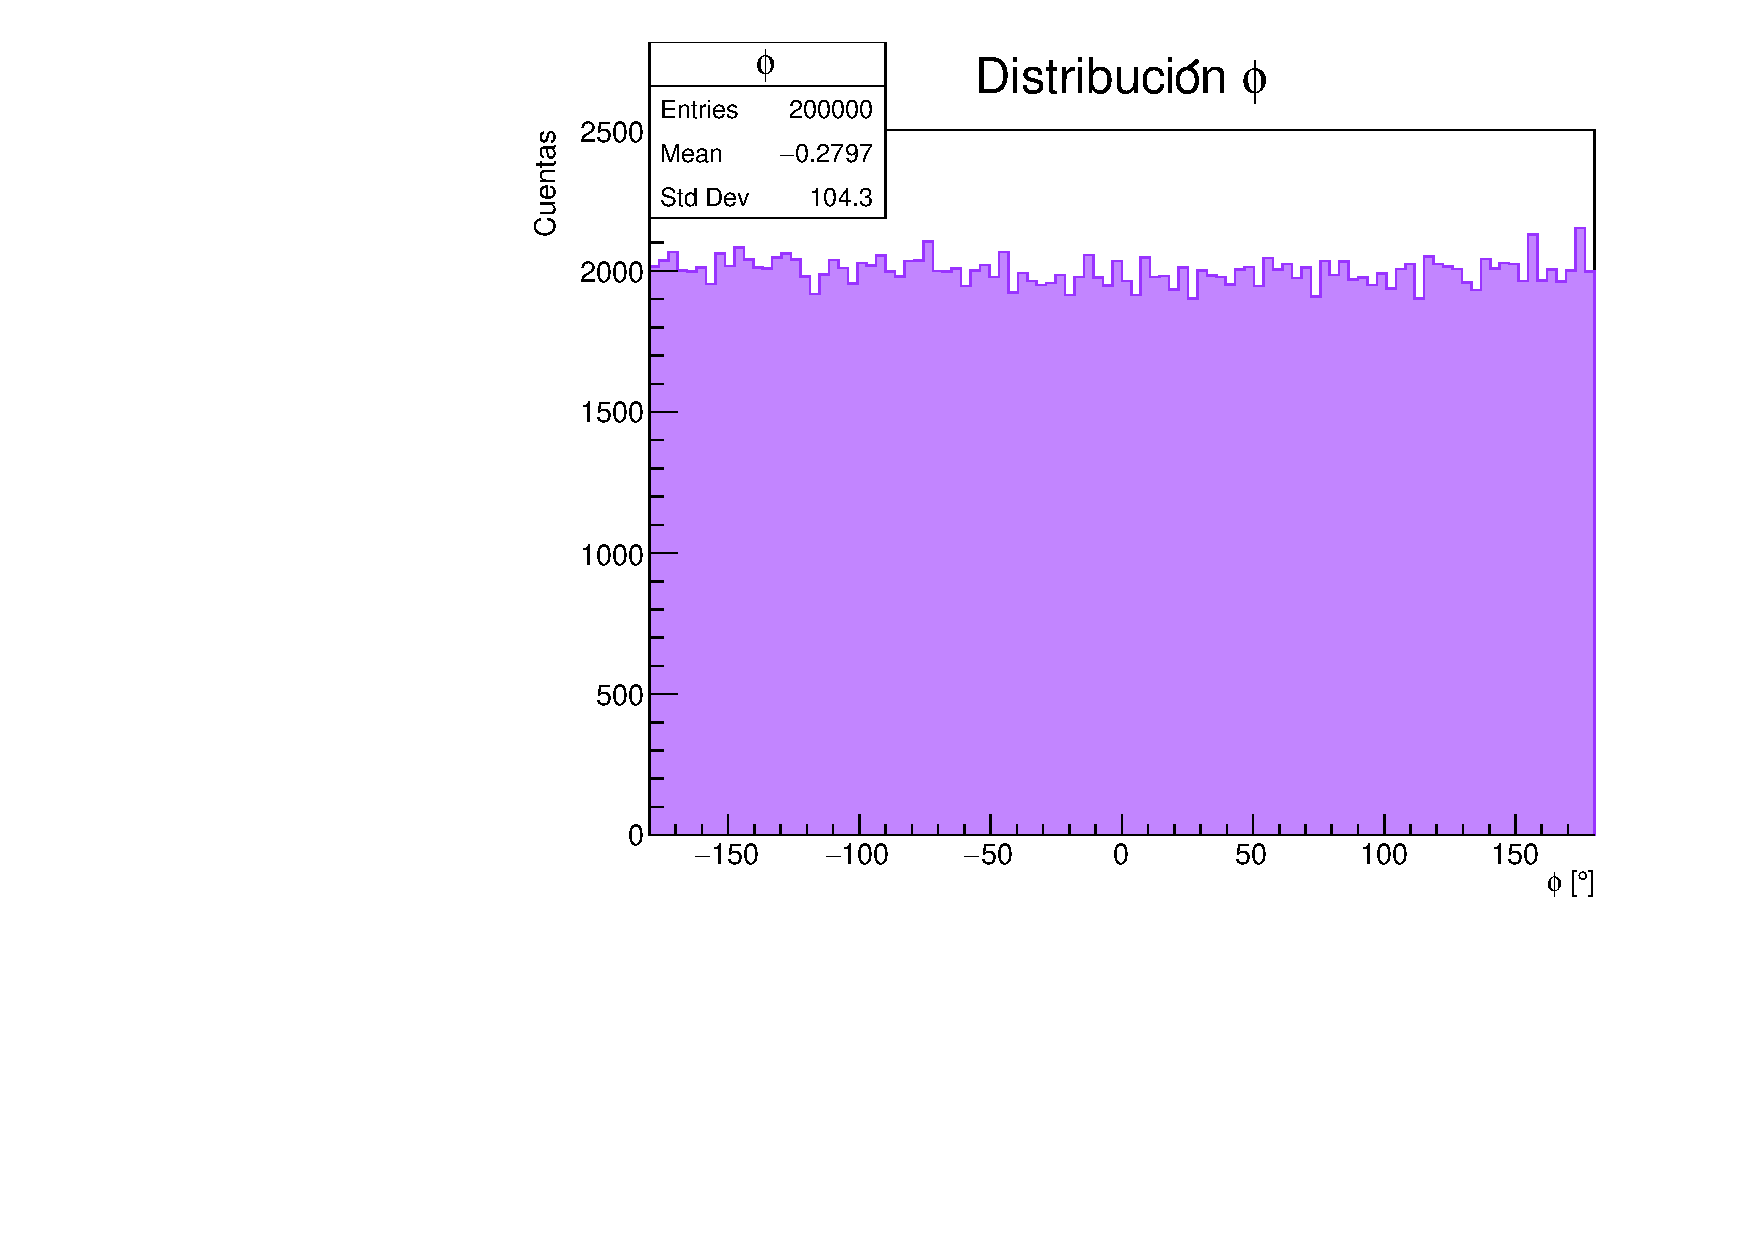
\includegraphics[width=0.8\textwidth]{../Figuras/Prob1B.pdf}}
\caption{Distribuciones de $\phi$ y de la pseudorapidez del muón.}
\label{fig:Prob1A}
\end{figure}
%%%%%%%%%%%%%%%%%%%%%%%%%%%%%%%%%%%%%%%%%%%%%%%%%%%%%%%%%%%%%%%

\textbf{2)}
\begin{figure}[H]
\centering
\subfloat[]{
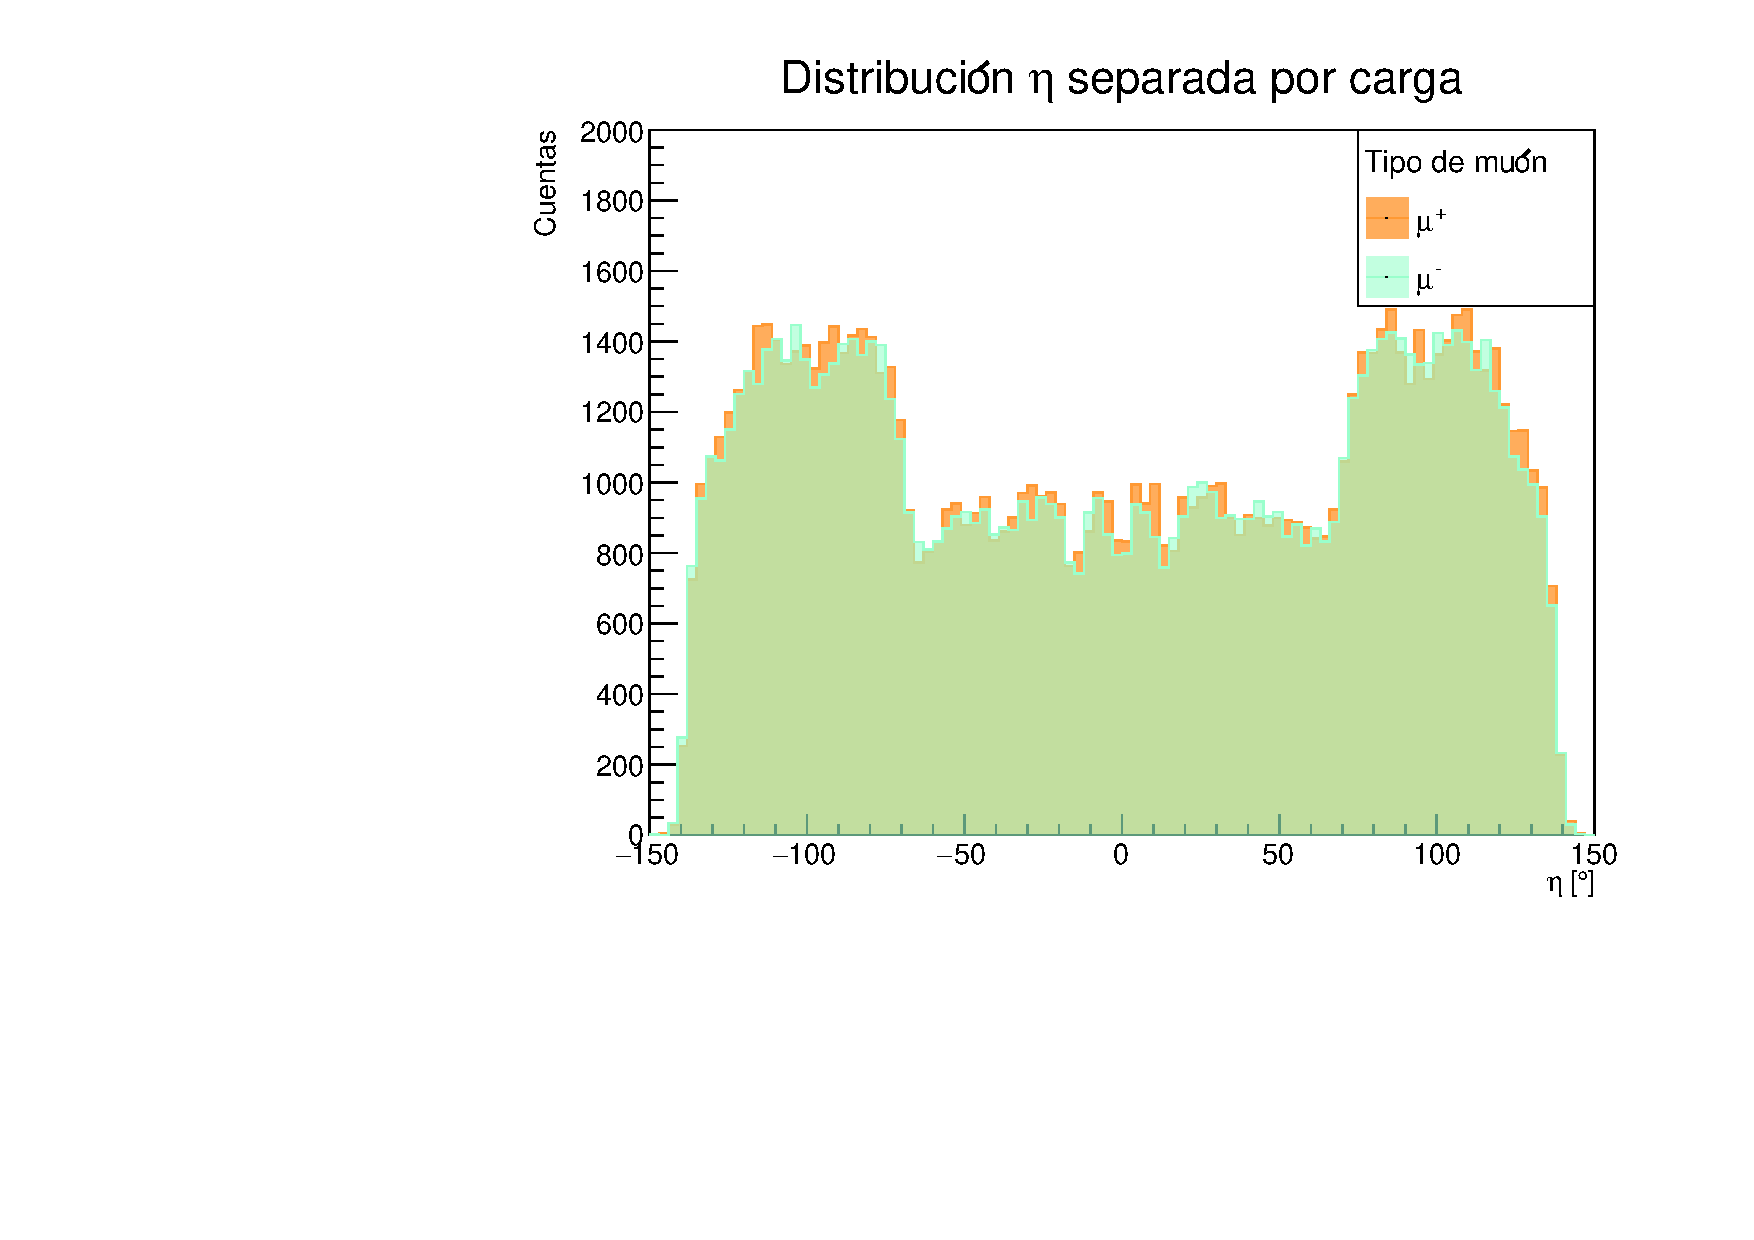
\includegraphics[width=0.78\textwidth]{../Figuras/Prob2A.pdf}}

\subfloat[]{
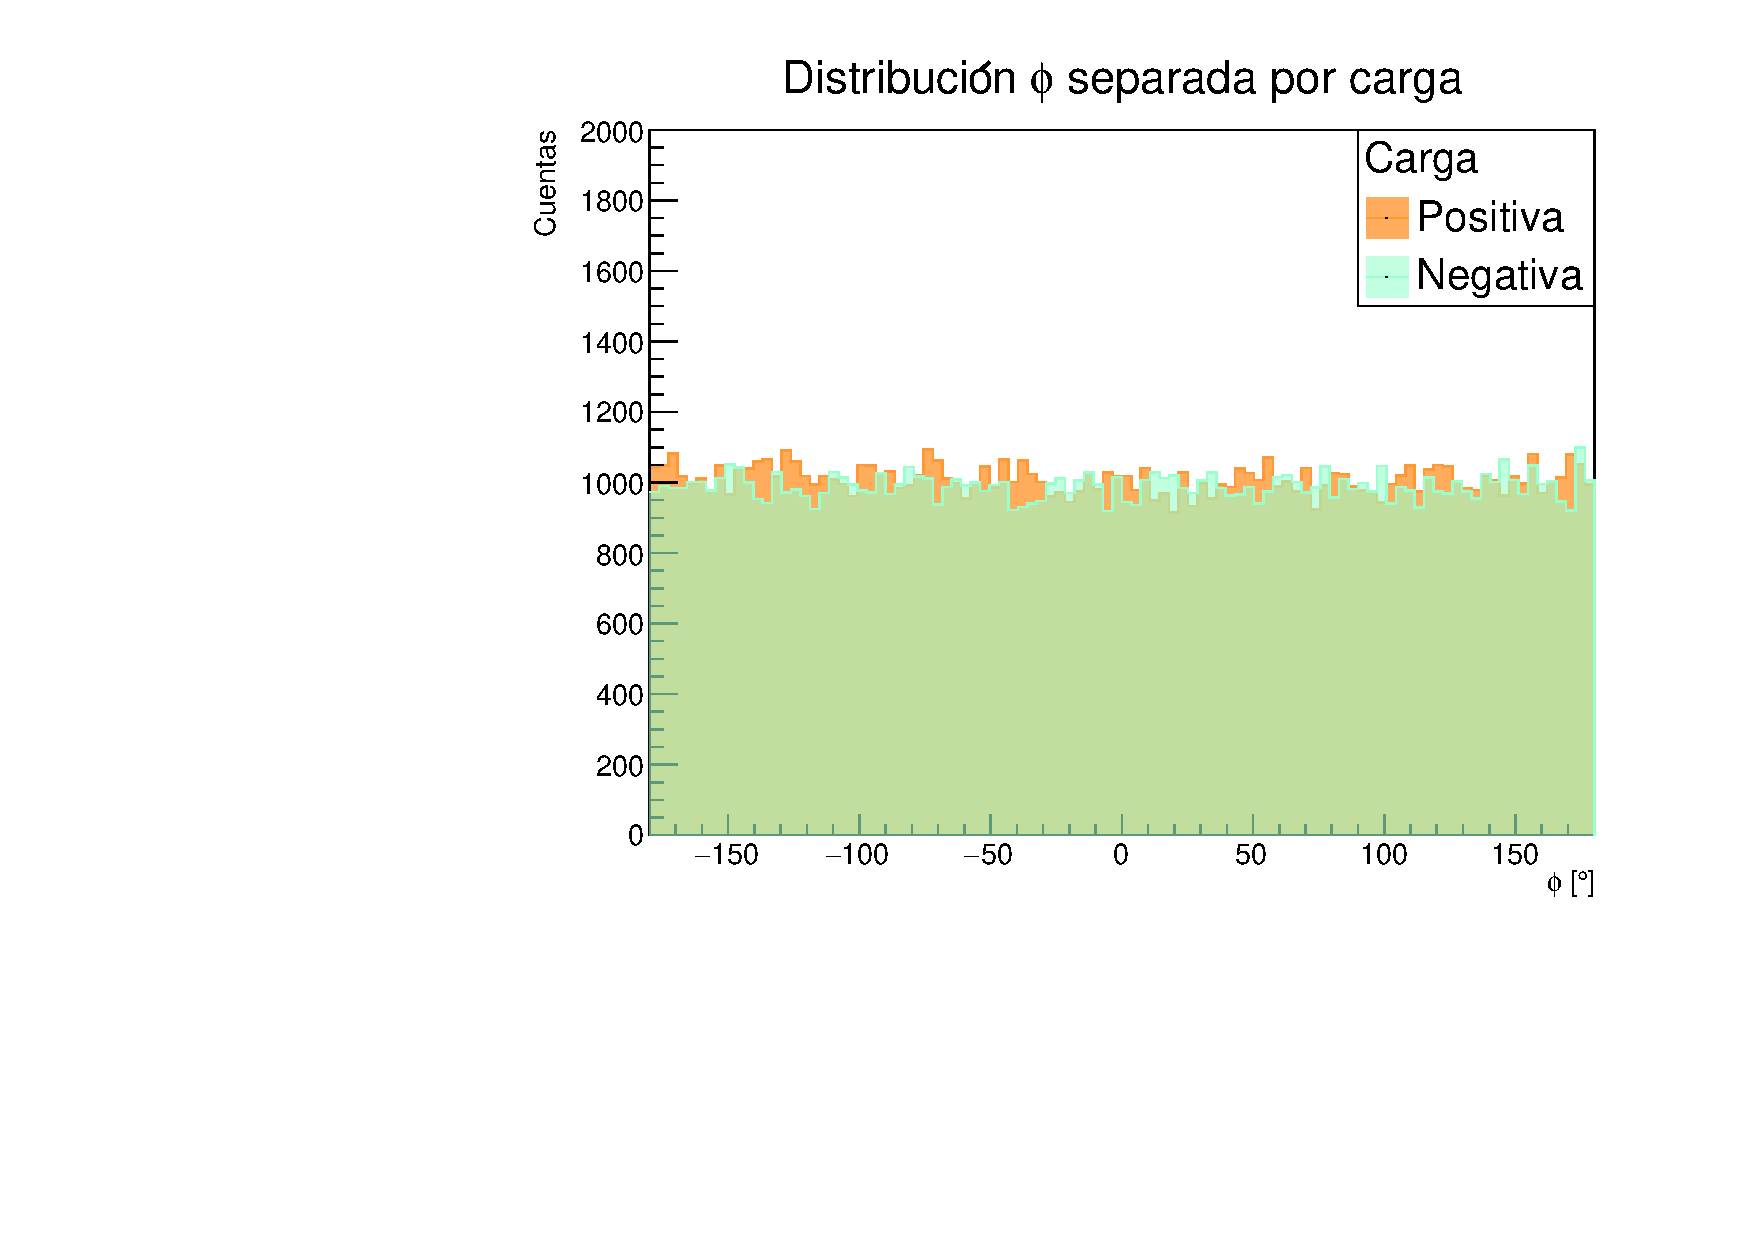
\includegraphics[width=0.78\textwidth]{../Figuras/Prob2B.pdf}}
\caption{Distribuciones de $\phi$ y de la pseudorapidez del muón separando por carga positiva y negativa.}
\label{fig:Prob2}
\end{figure}
%%%%%%%%%%%%%%%%%%%%%%%%%%%%%%%%%%%%%%%%%%%%%%%%%%%%%%%%%%%%%%%

\begin{figure}[H]
\centering
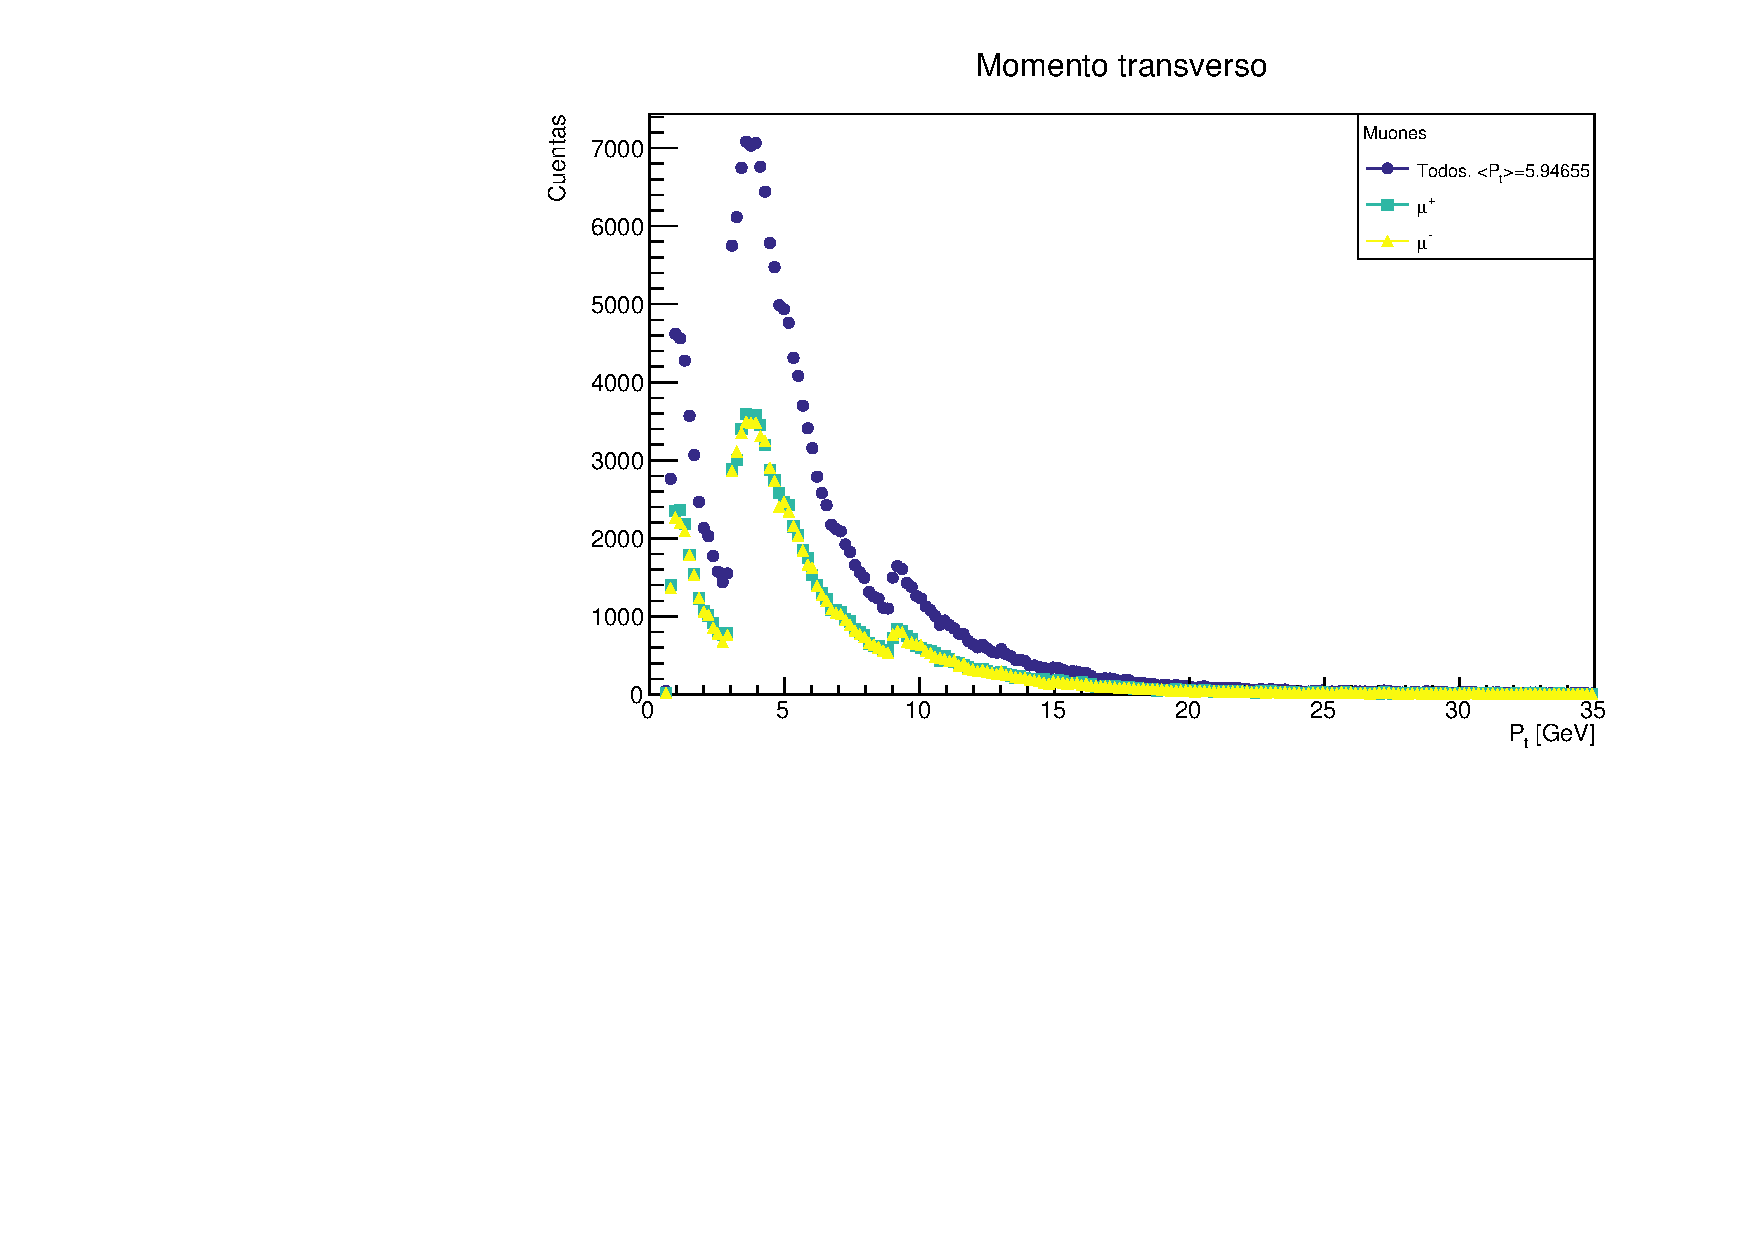
\includegraphics[width=1\textwidth]{../Figuras/Prob3.pdf}
\caption{Momento transverso para ambas cargas y haciendo la separación para positiva y negativa.}
\label{fig:Prob3}
\end{figure}

\pagebreak


\begin{figure}[H]
\centering
\subfloat[]{
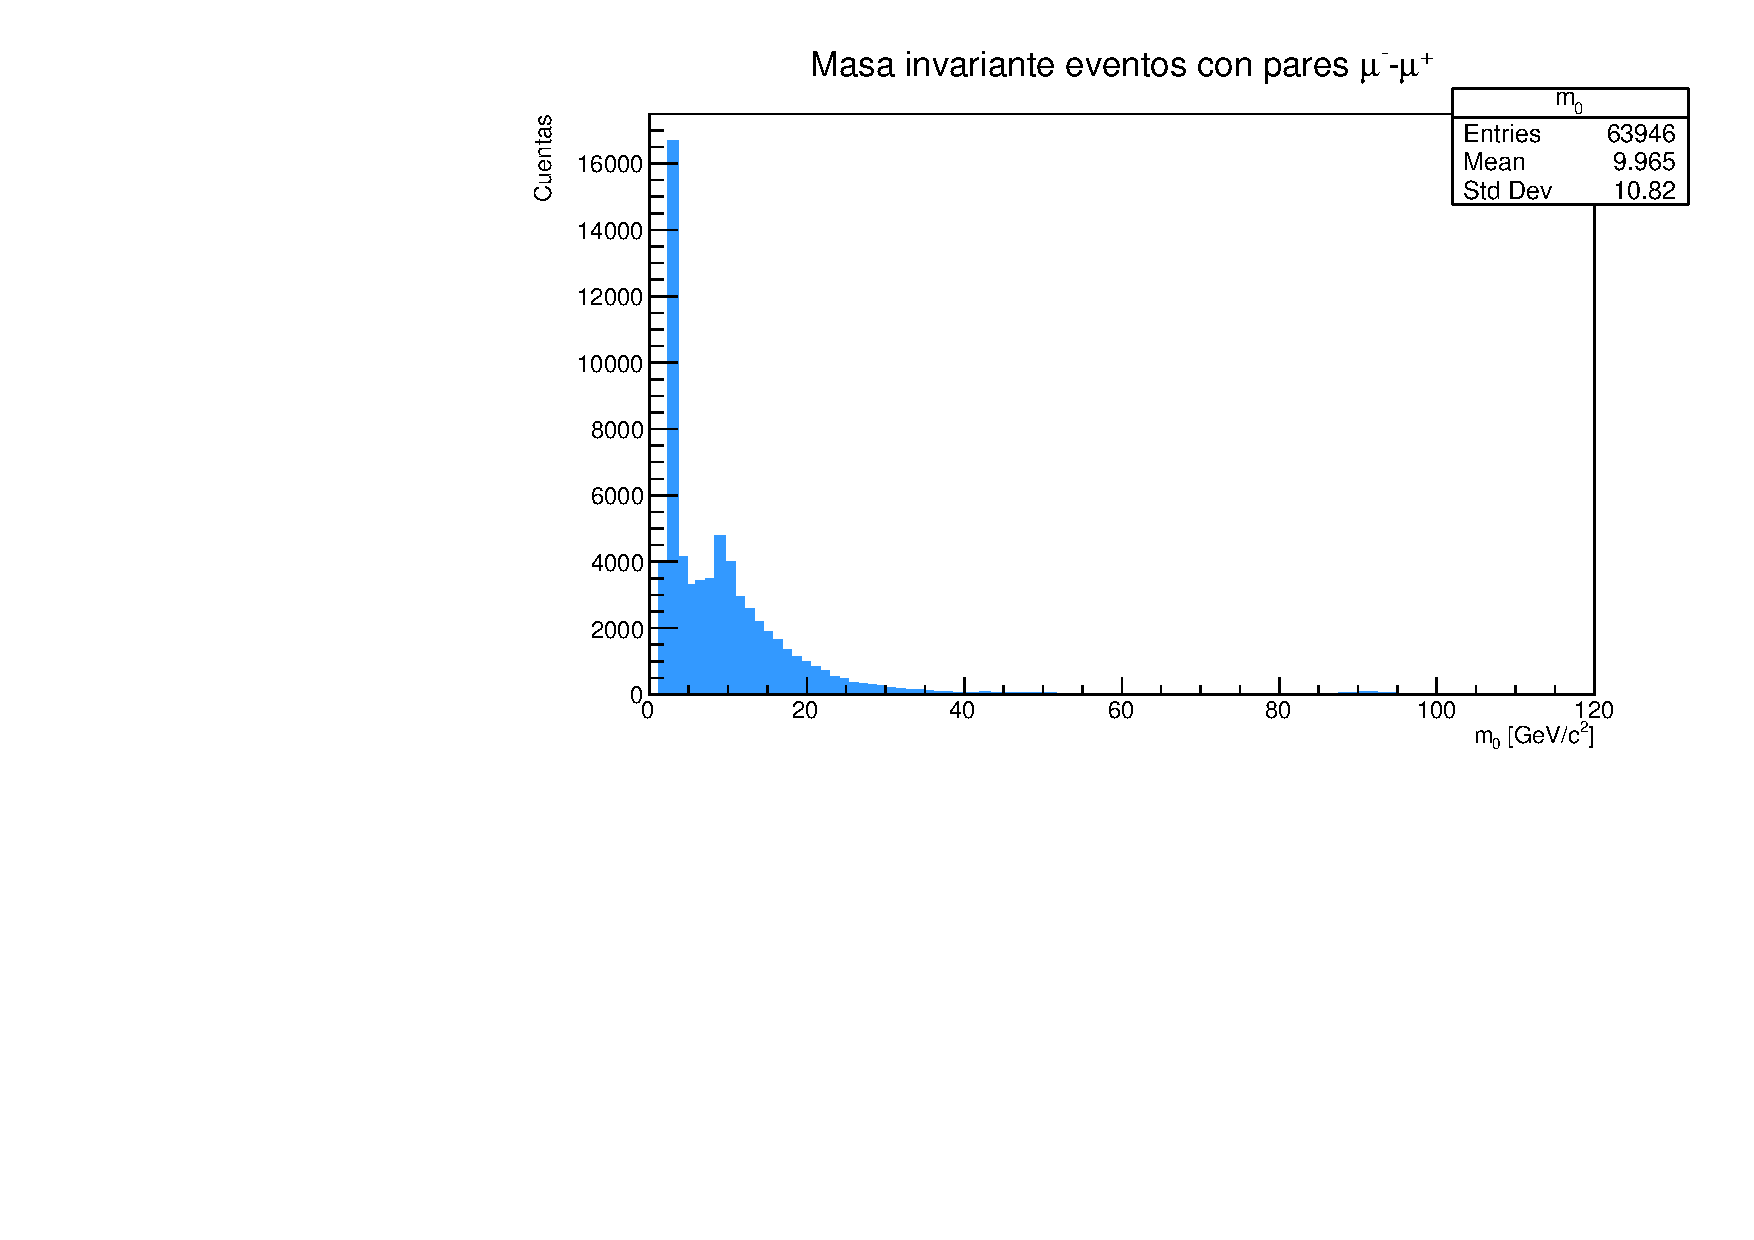
\includegraphics[width=0.78\textwidth]{../Figuras/Prob4A.pdf}}

\subfloat[]{
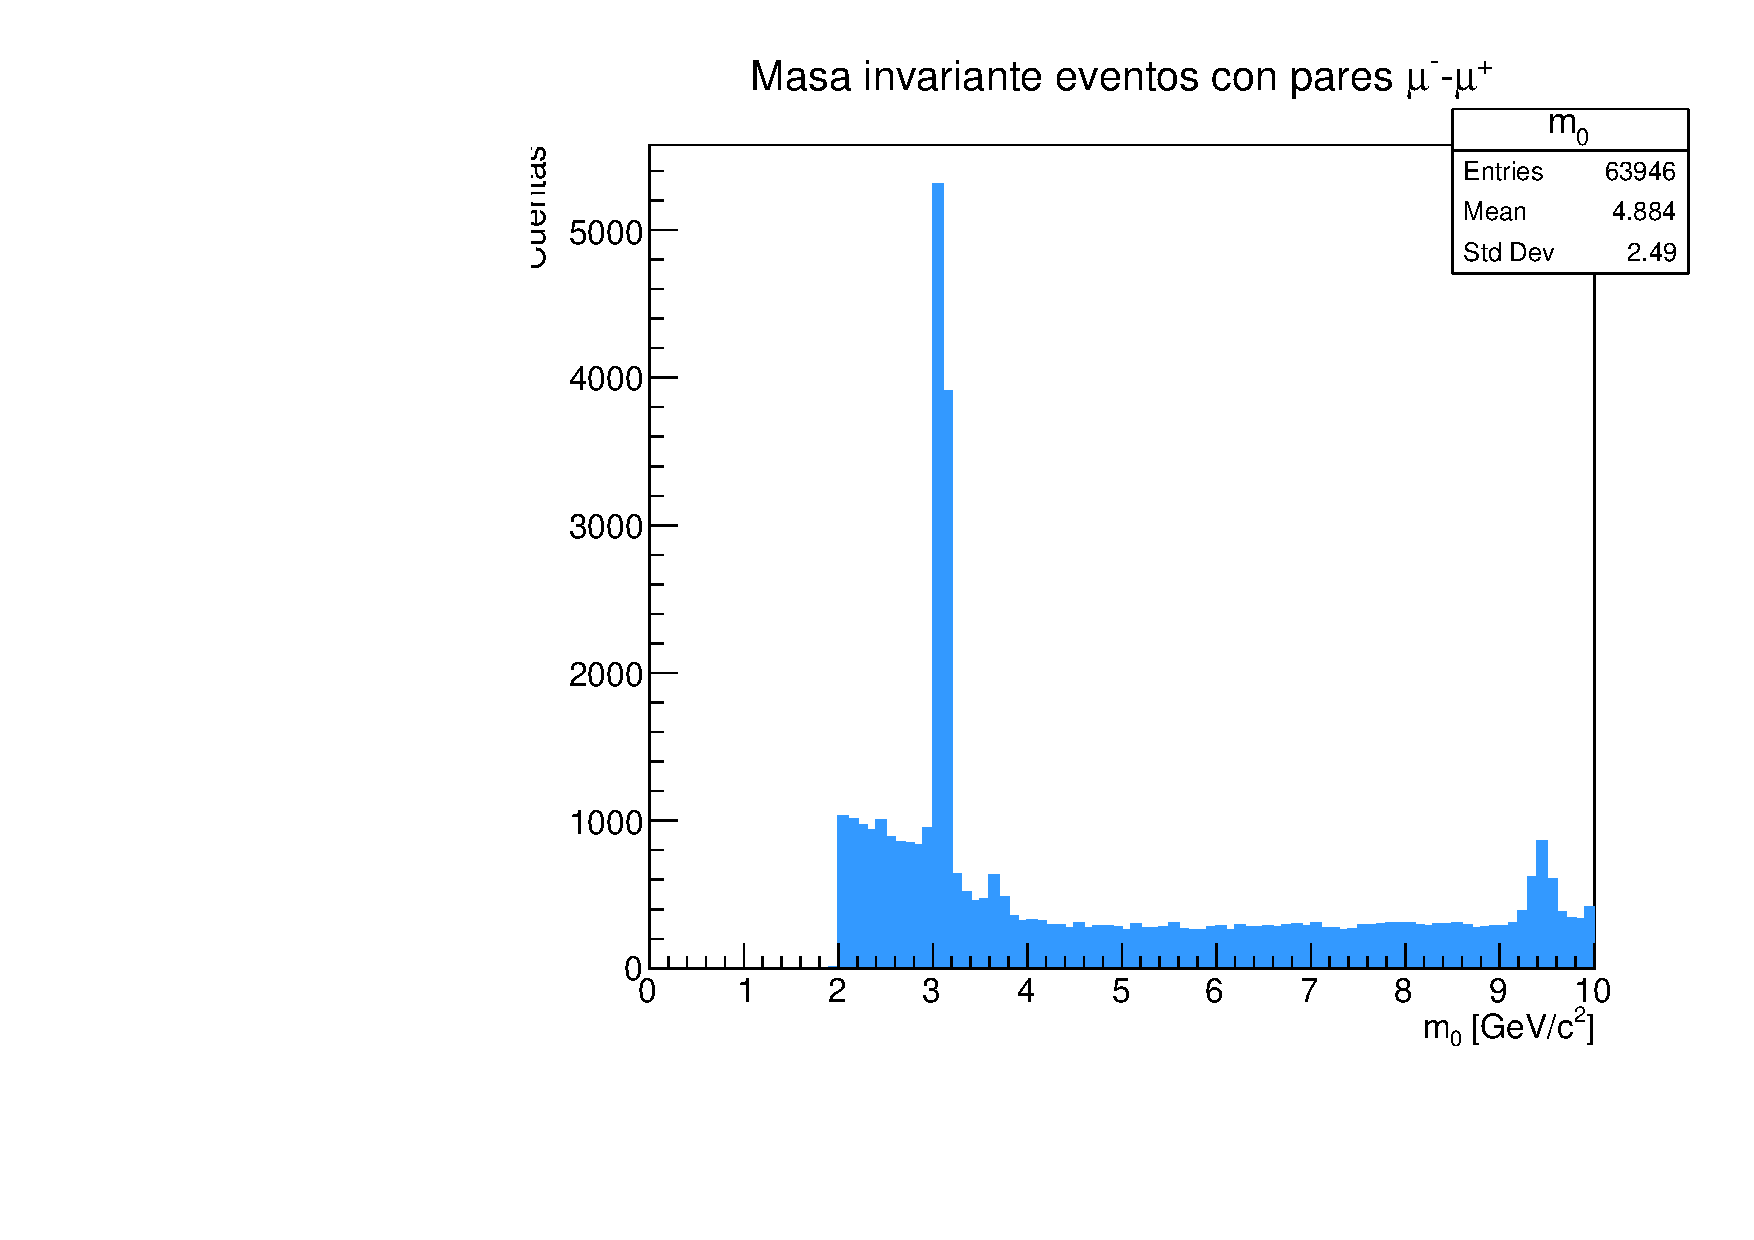
\includegraphics[width=0.78\textwidth]{../Figuras/Prob4B.pdf}}
\caption{Distribución de la masa en reposo para eventos donde únicamente haya un muón y un antimuón.}
\label{fig:Prob4}
\end{figure}

Podemos identificar al pico que está cerca de 3 GeV/$c^2$ como la partícula $J/\psi$, que decae en muones y además tiene una masa de 3.096 GeV/$c^2$.


\end{document}